% !TEX program = xelatex
%Wzór dokumentu
%tu zmień marginesy i rozmiar czcionki
\documentclass[a4paper,10pt]{article}
\usepackage{inputenc}[utf8]
\usepackage[margin=2cm]{geometry}
\usepackage{multicol}
\usepackage{graphics}
\usepackage{float}
\usepackage{tikz}
\usepackage{hyperref}
\hypersetup{
    colorlinks=false,
    linkcolor=blue,
    filecolor=magenta,      
    urlcolor=cyan,
    pdfpagemode=FullScreen,
    }
	\usetikzlibrary{arrows}
\usepackage{fancyhdr}
\pagestyle{fancy}
\fancyhead{}
\fancyfoot{}

\rfoot{\thepage}
\renewcommand{\headrulewidth}{1pt}
\renewcommand{\footrulewidth}{1pt}

\title{A way to investigate the soundscape of urban spaces: a case study on the example of city of Zabrze}
\author{
    Waldemar Paszkowski \\
    Silesian University of Technology, Gliwice, Poland, waldemar.paszkowski@polsl.pl
  \and 
    Artur Kuboszek \\
    Silesian University of Technology, Gliwice, Poland, artur.kuboszek@polsl.pl
  \and 
    Marcin Sobota \\
    Silesian University of Technology, Gliwice, Poland, marcin.sobota@polsl.pl
  \and 
    Marcin Dąbrowski \\
    Silesian University of Technology, Gliwice, Poland, marcin.dabrowski1@arcelormittal.com
  \and 
    Grzegorz Koperwas \\
    Silesian University of Technology, Gliwice, Poland, admin@grzegorzkoperwas.site
  \and 
    Kamil Kowalczyk \\
    Silesian University of Technology, Gliwice, Poland, kamil.kowalczyk.dev@gmail.com
  \and 
    Agata Fąfara \\
    Silesian University of Technology, Gliwice, Poland, agatfaf059@student.polsl.pl
  \and 
    Agnieszka Majda \\
    Silesian University of Technology, Gliwice, Poland, agnimaj205@student.polsl.pl
  \and 
    Sebastian Giełżecki \\
    Silesian University of Technology, Gliwice, Poland, sebagie167@student.polsl.pl
  \and 
    Wiktoria Paulus \\
    Silesian University of Technology, Gliwice, Poland, wiktpau727@student.polsl.pl
}

\date{29-30 November 2022}

\begin{document}

\maketitle

\thispagestyle{fancy}

\begin{abstract}
The paper describes the concept of design research on the soundscape in selected
places of the urban environment and presents the achieved results of the project
related to that. The method of acquiring and processing information about the
soundscape and its evaluation has been obtained by means of psychoacoustic tests
realized in laboratory conditions. An important element of the carried out
research was the development of an application that shares soundscape map
information to users using mobile technologies. The application allows
identification and assessment of city soundscape.
\end{abstract}


\section*{Introduction}

\begin{multicols}{2}

The assessment of noise pollution in the outdoor spaces is one of the complex
problems related to environmental assessment. In order to perform this kind of
assessment the sound sources and parameters characterizing acoustic climate have
to be investigated. Variability of these parameters is mainly due to the type
and dynamics of sound sources over time and instability of meteorological
conditions.  The specificity of noise pollution lies in the complexity of human
hearing and its subjective evaluation, in the high spatio-temporal variability
and in the rich spectral content of noise generated by a variety of sources in
the environment.

In terms of describing the acoustic environment and evaluating noise mitigation
strategies, relevant noise indicators have to be used. Correct selection of
appropriate noise indicators in the urban context and making decisions based on
them is a necessary activity when it comes to the threat mitigation of noise
sources.

Research on noise indicators has led to the conclusion that $L_{Aeq}$ has been
recognized as a basic descriptor for evaluating sounds, including fluctuating
ones.

The $L_{Aeq}$ indicator is critically evaluated in many respects, including:
\begin{itemize}
    \item it is not the best indicator for assessing pleasant sounds,
    \item it covers only the energy dimension of noise, and therefore poorly
    distinguishes between sound environments.
\end{itemize}

It should be noted that the various energy indicators used for noise annoyance
assessment do not take into account the evaluation of fluctuating sounds, which
are commonly found in urban areas and which have a negative impact on noise
  annoyance \cite{Schomer:2005}.

According to the studies on the identification of the soundscape, its occurrence
in human perception in the acoustic environment is considered as the basis for
  its existence \cite{Brown:2010}. The soundscape depends strongly on human perception in the
context of a specific time, place and activity. The soundscape refers to the
perception aspect of preferred sounds.

Attempts to correlate objective and subjective information obtained from
environmental and laboratory studies are an important source of knowledge on the
soundscape. In particular, the acquisition of objective information includes
``in-situ'' measurements of sound levels, binaural sound recordings and sound
characteristics. The use of methods linking acoustic comfort to sound levels,
mainly by means of $L_{Aeq}$, is increasingly important in the implementation of
soundscape research work, particularly in the assessment of urban noise.

In the studies on the soundscape and its impact on people's daily lives as well
as psychological and health aspects, three basic approaches can be considered,
i.e. physical, psychophysical and perceptual:
\begin{itemize}
    \item \textbf{the physical approach} adopts an objective assessment of the acoustic
      environment \cite{Directive:2002/49}. This approach utilizes the technology of acoustic mapping,
    which is a basic tool in the tasks of assessing and forecasting the acoustic
    environment of a large part of European countries. In this approach,
    acoustic impressions of sound perception are treated secondarily,
    \item \textbf{psychophysical approach}, includes the relationship between the
    acoustic environment and the impressions of sound perception. Objective
    acoustic parameters (i.e., most often in the form of sound levels) are
    linked to subjective impressions of acoustic evaluation. The complexity of
    this approach lies, among other things, in the direct consideration of
    varying sound characteristics (represented in the time and frequency
    domains) and personal or socio-demographic
    characteristics \cite{Booteldooren:2006, Weinstein:1980}. 
    \item \textbf{The perceptual approach} has relatively recently begun to be taken into
    account, in this case the soundscape is treated mainly as a source of
    information and an element of the interaction between people and the
    environment.
\end{itemize}


Among the methods used to assess the soundscape the following are worth
mentioning \cite{Ozcevik:2008}: 
\begin{itemize}
    \item analysis of acoustic signals under laboratory conditions,
    \item the sound walk method,
    \item the survey research method.
\end{itemize}
Analysing acoustic signals under laboratory conditions, targeting the perception
of the sound environment is one of the methods evaluating the soundscape that
can be useful in obtaining more information when comparing to the typical
environmental studies. This method provides exposure to the sound environment in
established and controlled situations. The ability to use ambisonic technology
allows for a relatively accurate synthesis of the sound field through the use of
a multi-channel listening system. Analyses from the resulting signals are used
to search for coefficients that characterize the soundscape.

The sound walk method is used in soundscape analyses and evaluations, such as
the study of locations on the pedestrian path. This method includes measurements
of psychoacoustic indicators and evaluation of people's perceptions at the
locations under study. One of the goals of using the sound walk method is to
look for correlations of psychoacoustic parameters for each location, in order
to determine the strength of the relationship between objective parameters and
soundscape perception.

The survey research method uses a survey form consisting of two parts: \emph{a
questionnaire} and \emph{a semantic differential test}. 

The \emph{questionnaire part} includes categories such as personal information,
land use, compliance with expectations and evaluation of the environment in
terms of examining pleasant impressions of the soundscape.

The \emph{semantic difference test} is used to examine the quality of the
soundscape environment. The pairs of adjectives that are used in the semantic
difference test are selected according to the native language of the related
community and the soundscape description aspects.

It should be noted that the focus of the research on developing the idea of
soundscapes for environmental noise assessment can contribute to the
understanding of human response to noise sources in both urban and non-urban
areas.

In the 2021/2022 academic year, the research works portfolio of the
\emph{Silesian University of Technology} includes PBL \footnote{Project
Based Learning} projects. In particular, a project entitled \emph{``Designing
the acoustic component of a smart city using the concept of soundscape and
mobile technologies''}, which has been carried out by an interdisciplinary and
an interdepartmental team of students and academics, in particular: the
\emph{Department of Organization and Management} and the \emph{Department of
Applied Mathematics}. The problem addressed in the project concerns aspects of
designing the soundscape of urban spaces, with a particular focus on the
interaction of the citizens with the acoustic stimuli present. The formulated
title of the project is in line with the development and implementation of the
\emph{SmartCity 3.0} concept in the cities. Solving the problem requires the
development of a method to study the city soundscape using appropriate models,
procedures and tools for recording, collecting and accurate processing of the
acoustic signal. The starting point for developing a soundscape creation method
is the procedure of creating strategic noise maps using the concept of layered
map implemented in GIS\footnote{Geographic Information System} and the latest
international standards for soundscape identification and analysis
\cite{ISO:12913-1, ISO:12913-2, ISO:12913-3}.

In order to identify and assess the acoustic climate of the cities, the
strategic noise maps are being created. Based on the current EU Directive
2002/49/EC the strategic noise maps are prepared for four classes of noise
sources: road noise, rail noise, aircraft noise and industrial noise. It should
be noted that strategic noise maps are prepared for the purpose of assessing and
preventing noise pollution caused only by the above-mentioned sources. In
reality, the problem becomes more complicated and complex, as urban spaces are
also exposed to diverse sources with varying dynamics, both natural and
anthropogenic sources. The concept of soundscapes, which is being developed in
environmental acoustic research, includes various aspects and factors related to
sound perception in particular. Reducing the assessment of life quality only to
one criterion, which is the human perception of the particular place (including
sound perception), consequently leads to the question: is it pleasant or
unpleasant to be in this place?

The results of studies on the phenomenon of noise confirm that the
psychoacoustic aspects of sound, the temporal structure of the signal, the
formation of subjective characteristics of sound in the following domains: time,
frequency, time-frequency, among others, have a significant impact on the
perception of noise \cite{Gaja:2003, Neibo:2013, Nilsson:2007}.

It was assumed that the soundscape creation methodology can be created by means
of designing two experiments:
\begin{itemize}
    \item in an outdoor environment: recording and processing of the acoustic
    signal using specialized measurement equipment,

    \item in a closed room: evaluation of the acoustic signal using a listening
    booth and the psychoacoustic test method.
\end{itemize}

It should be noted that it is currently impossible to distinguish pleasant and
unpleasant sounds using dedicated equipment, because there is a lack of such
solutions both in the area of the use of appropriate measurement methods and the
implementation of appropriate technologies.

Modern digital technologies in conjunction with appropriate modeling solutions
make it possible to effectively support design tasks. The advantage of digital
technology applications is the ability to support decision-making in both the
short and long-term horizons with direct public participation. It therefore
becomes crucial to develop a way of acquiring, collecting, processing and
sharing digital information in the creation of smart solutions for the cities.
Currently a Smart City is a city that uses advanced information and
communication technologies more consciously, interactively and efficiently
\cite{Manville:2014}.

It was assumed for the implementation of the research that the collected
acoustic signal measurement data set represents various sound sources of natural
and anthropogenic origin.

The tangible result of the project was the development of an application for
mobile devices, that allows users to identify and evaluate the soundscape for
selected points on the city map.

\end{multicols}

\section{Description of the research concept}

\begin{multicols}{2}

The research area considered in the project can be identified with the help of
relationships and interactions occurring among: the environment, sound source(s)
and humans. The developed concept of soundscape, which is based on the
identification and evaluation of sound perception, corresponds to contemporary
challenges and needs of acoustic design of smart cities.

Taking into account the subjective aspects of evaluating different sounds with
respect to (but not limited to): the place of residence, the activities carried
out, the nature and duration of the acoustic stimulus, as well as other factors
accompanying the perception of sound, are of key importance in the tasks of
designing the city's soundscape.

In the adopted concept for the implementation of design tasks, it was assumed
that soundscape research will use:
\begin{itemize}
  \item acoustic and aural signals as sources of sound information of the
    environment,
  \item GIS models and tools as a way of representation and processing of sound
    information (the basis of the GIS spatial data model is a set of geometric
    elements in raster or vector form, i.e.: points, lines, surface objects,
    which are used to represent real world objects; geometric objects are stored
    on thematic layers, connected to tables containing descriptive attributes,
    characterizing them qualitatively or quantitatively),
  \item mobile application solutions that allow the acquisition and sharing of
    environmental sound information using mobile devices.
\end{itemize}

Known methods of digital acoustic/phonic signal processing use advanced models
and techniques for its evaluation. They allow the study of the soundscape of
urban spaces by means of physical features and auditory impressions of sound,
fig. \ref{processing}.

\end{multicols}
\begin{figure}[H]
  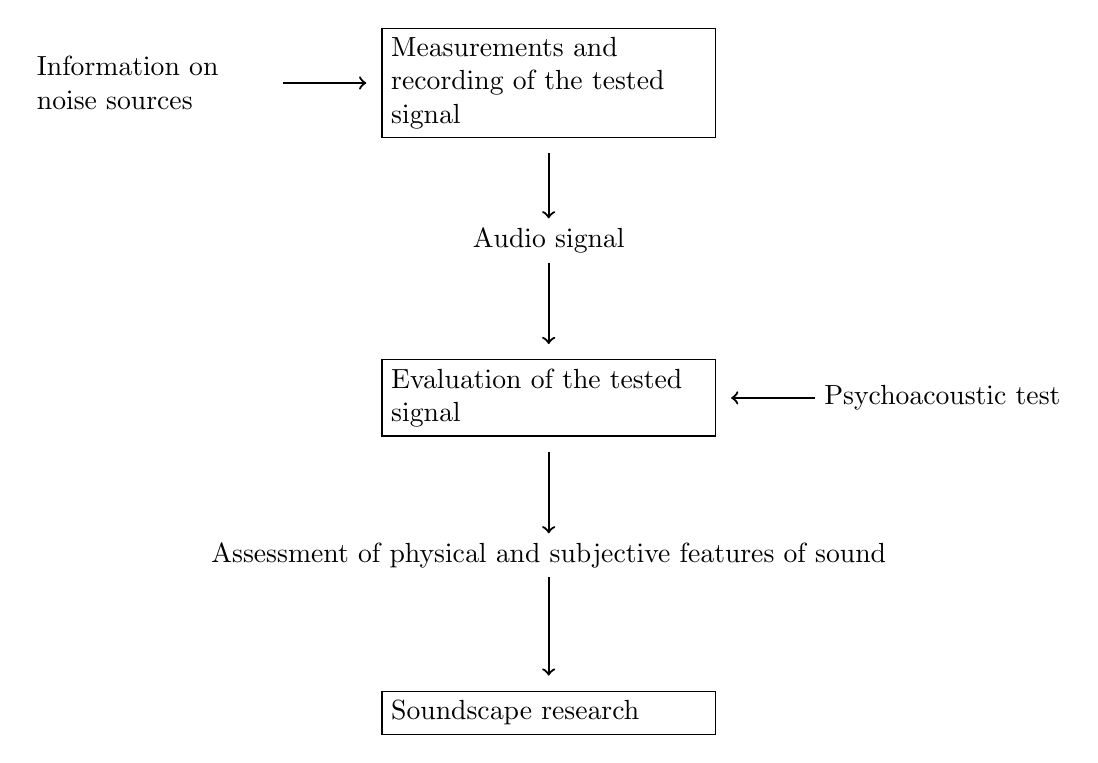
\begin{tikzpicture}[auto=left]
    \node (A) [text width=3cm,anchor=center] at (-1, 0) {Information on noise sources};
    \node (B) [text width=4cm, draw, anchor=center, outer sep=2mm] at (4, 0) {Measurements and recording of the
    tested signal};
    \node (C) [anchor=center] at (4, -2) {Audio signal};
    \node (D) [text width=4cm, draw, anchor=center, outer sep=2mm] at (4, -4) {Evaluation of the tested signal};
    \node (E) [anchor=center] at (9, -4) {Psychoacoustic test};
    \node (F) [anchor=center] at (4, -6) {Assessment of physical and subjective
    features of sound};
    \node (G) [text width=4cm, draw, anchor=center, outer sep=2mm] at (4, -8) {Soundscape research};
    \draw[->,thick] (A) edge (B);
    \draw[->,thick] (B) edge (C);
    \draw[->,thick] (C) edge (D);
    \draw[->,thick] (E) edge (D);
    \draw[->,thick] (D) edge (F);
    \draw[->,thick] (F) edge (G);
  \end{tikzpicture}
  \centering
  \caption{General scheme of information acquisition and processing for the
  study of the soundscape of urban spaces}
  \label{processing}
\end{figure}

\begin{multicols}{2}

For the soundscape study (Fig. \ref{processing}), the following steps were
  taken:
\begin{itemize}
  \item measurement and recording of the acoustic signal, which is the starting
    point for processing information about the characteristics of the acoustic
    and phonic signal,
  \item evaluation of the registered signal, involving methods and techniques
    that allow listeners to assess the annoyance/pleasantness of the sound of
    the registered signal, using the psychoacoustic test method.
\end{itemize}

The location of points where acoustic measurements are made and sounds are
  recorded, plays a key role in the study of the soundscapes. In order to
  properly map the measurement points, the project uses a layered model,
  implemented in geographic information systems (GIS). In the adopted model, the
  visualization part is a set of points located on a map base (raster layer),
  representing the locations of the measurements. In turn, the descriptive part
  of this layer contains a set of attributes characterizing aspects related to
  the acoustic measurements themselves (recorded equivalent sound level
  $L_{Aeq}$, temperature, humidity and atmospheric pressure at the time of the
  measurements). The descriptive attributes are stored in the database. At a
  given measurement point, they are available in the application based on their
  individual ID. In addition, this collection of points has been supplemented
  with photographs of the measurement sites and audio files of the audio
  recording made during the measurement. The \texttt{FastAPI} framework and the
  \texttt{React.js} library were used to create the interface of the mobile
  device application visualizing the information assigned to the surveyed
  points.

The data representation structure prepared in this way was the starting point
for collecting data from measurements taking into account physical and
subjective characteristics of sound.

\end{multicols}
\section{Measurements and recordings of the acoustic signals as a source of
  information about the soundscape}

\begin{multicols}{2}

  A key aspect to the implementation of the listening study was the creation of
  the broadest possible base of sounds in the outdoor environment. To achieve
  this goal - sound registrations were carried out with simultaneous measurement
  of sound pressure levels.

  To carry out the registration and acoustic measurements, 3 devices were used:
  \begin{itemize}
    \item SVAN 945A sound level meter,
    \item Two ZOOM sound recorders.
  \end{itemize}

  One of the sound recorders (ZOOM model H3-VR) has an ambisonic recording
  option thanks to the four microphones it contains, which allows recording
  surround sound from all sides simultaneously. The recordings were made with
  the AmbiX feature, as a result the audio can be played back in Ambisonics B
  format on four channels, which was also important for further psychoacoustic
  tests.

  Measurement of sound pressure levels at selected points in the city was an
  important part of the research for the implementation of psychoacoustic tests.
  These values allowed calibration of the listening equipment involving
  re-measurement of sound pressure levels under laboratory conditions. Proper
  provision of sound levels during the listening tests in the amplification
  setting of the amplifier made it possible to adequately represent the
  immission of sound sources and provide acoustic conditions occurring during
  the implementation of measurements.

  The sound recorders were the main tools for recording the audio signals under
  study. They were equipped with additional tripods, keeping the devices at a
  certain height, which made it possible to minimize the phenomena of reflection
  and absorption of sound by members of measurement team.

  The sound recordings consists of 60-seconds of acoustic signal samples for
  each measurement point. The sampling frequency of the recordings was set at
  44.1kHz. The frequency adopted is primarily due to the maximum frequency of
  human hearing - 20kHz, the Kotielnikov-Shannon theorem and the Nyquist
  frequency. On the one hand this frequency was a compromise due to the fact,
  that the evaluation of auditory impressions of sounds for most participants
  will not differ with increased sampling frequency. On the other hand,
  increasing the sampling frequency would significantly increase the amount of
  recorded data \cite{ISO:266, ISO:9613-1}.

  Measurement of sound pressure levels at the test points were also carried out
  for 60-seconds. The obtained measurement value, recorded and saved in the
  application, was the $L_{Aeq}$ value. The measurement was carried out with
  filter A and FAST characteristics on. Sample data recorded at a particular
  measurement point are shown in fig. \ref{exampleData}.
\end{multicols}

\begin{figure}[H]
  \includegraphics[scale=.5]{fig2.png}
  \centering
  \caption{Example data recorded at the measurement point}
  \label{exampleData}
\end{figure}

\begin{figure}[H]
  \includegraphics[scale=.9]{fig3.png}
  \centering
  \caption{Example view from the measurement database}
  \label{exampleView}
\end{figure}

\begin{multicols}{2}

  The dedicated mobile application was used for collecting measurement data and
  additional attributes directly in the measurement point, (Fig.
  \ref{exampleView}). The developed application allows to capture the following
  information related to the measurement: the name and description of the
  measurement point, comments, tags, $L_{Aeq}$ index values and a photo
  identifying the measurement point. The collected data at the measurement point
  are transferred to the measurement database, which is additionally
  supplemented with recorded sound sample files.

  Additional information that is recorded during the measurements (Fig. \ref{finalUI}) is
  the weather data including temperature, pressure and humidity. Although the
  values of these parameters did not fluctuate significantly, with careful
  analysis it is possible to study the relationship between this weather
  parameters and sound pressure levels and how the acoustic signal is evaluated
  by listeners \cite{Neibo:2013}.

\end{multicols}

\begin{figure}[H]
  \includegraphics[scale=.9]{fig4.png}
  \centering
  \caption{An excerpt from the map with sample information on the measurement point}
  \label{finalUI}
\end{figure}

\begin{figure}[H]
  \includegraphics[scale=.5]{fig5.png}
  \centering
  \caption{A section of the city area with the location of the measurement points}
  \label{finalMap}
\end{figure}

\begin{multicols}{2}
The application provides an automatic backup in the cloud functionality as well
  as allows to correct potential errors entered during the measurement process.

  Sound measurements and recordings were carried out in 60 selected measurement
  points (Fig. \ref{finalMap}, Fig. \ref{finalTable}). The selection of measurement points has being
  determined by their spatial location, their proximity to particular buildings
  or elements of the surrounding area, and the likelihood of a characteristic
  sound in the area.

  For example in the urban spaces intended for educational purposes - some
  characteristic sounds for such places are expected, i.e.: noise caused by
  increased traffic, the voices of students, the sound of school bells, etc. In
  the case of the industrial sector, the characteristic signals are noises
  coming from production halls, sounds of the operation of technological and
  construction machinery, and sounds generated by workers. The points marked on
  the map can be also identified by a color designation, which corresponds to
  the average rating of sound samples obtained during psychoacoustic testing.
  The lower values of this evaluation are marked with reddish colors, while the
  higher values correspond to greenish colors.

  In the most cases, acoustic measurements were carried out during the day (from
  the morning to late evening hours), in order to capture characteristic sound
  sources in the studied urban spaces. It was assumed that increased sound
  levels would be observed during the afternoon hours, when traffic, school and
  industrial noise is more intense. Therefore, one of the criteria for the
  selection of measurement points was also the time period during which the
  measured signal could be most audible.
\end{multicols}

\begin{figure}[H]
  \includegraphics[scale=.3]{fig6.png}
  \centering
  \caption{The identification of measurement points}
  \label{finalTable}
\end{figure}

\begin{figure}[H]
  \includegraphics[scale=.7]{fig7.png}
  \centering
  \caption{Share of land use types in the total number of measurements}
  \label{finalChart}
\end{figure}

\begin{multicols}{2}
  Three main land use types dominate in the investigated area (Fig.
  \ref{finalChart}): the Industry, the Public Spaces and Parks. This indicates
  some variation in the purpose of the city's places, which are accompanied by
  the emission of characteristic acoustic signals.

  The smallest share occurred for the areas allocated to Services and Hospitals.
  This is due to the fact that these areas have relatively low sound pressure
  levels for most of the day. The main sources of sound outside buildings are
  vehicle's emergency sirens, which operate only in cases of danger to life and
  safety.

  The results obtained from the soundscape study allow to identify the acoustic
  characteristics city Zabrze - it is an area with a dominance of industrial
  business, where public space and areas for recreation form small parks and
  squares along with fountains \cite{Lewandowski:2008}. Probably these are not typical acoustic
  conditions of most cities in Poland. Therefore, it is reasonable to conduct
  this type of research in other agglomerations, which will allow to identify
  and assess the specifics of the soundscape. The information obtained from such
  studies can be used in local projects that will take into account people's
  behavior and their sound interaction with the environment.
\end{multicols}

\section{Evaluation of sound impressions using the psychoacoustic test method}

\begin{multicols}{2}
  Psychoacoustic tests are used in many research works oriented toward
  subjective evaluation of sound. Among other things, they are used for:
  determining metrics of sound quality and rotorcraft noise annoyance
  \cite{Krishnamurthy:2018}, assessing the quality of telephone transmissions
  \cite{ITU-T:P800}, or experimental studies of annoyance caused by acoustic
  signals from trams and buses \cite{Sandrock:2008}. 

  In a study on determining metrics of sound quality and annoyance from
  rotorcraft noise \cite{Krishnamurthy:2018}, a psychoacoustic test was
  conducted on 40 people who listened to 105 differently modified, six-seconds
  long samples of helicopter sound. Based on a five-point rating scale,
  individuals determined the irritation caused by the sound of the rotorcraft.
  The conclusion of this research was that the subjects' irritation was
  influenced not only by the loudness of the rotorcraft sound but also by other
  subjective characteristics of the sound, such as: sharpness, tonality and
  strength of fluctuations.

  The psychoacoustic test in the experimental study of annoyance, caused by car
  and bus noise, consisted of two parts. The first part of the experiment was
  based on 7 pairs of acoustic samples captured from cars and buses, each with a
  difference of 3dB. Research participants was listening to the samples and
  assessing of their annoyance reflected on an 11-point scale. In the second
  part the research participants were exposed to a 2-hour traffic scenario,
  during which they performed certain tasks. The result of the first test was
  that the noise of a car was described as equally annoying as the noise of a
  bus, which actually was 3 dB lower. The second part of the test concluded that
  both types of sounds had the same impact on task performance, with the noise
  signals from the car causing less annoyance during work.

  In the project undertaken by the authors of this paper, the evaluation of
  sound perception was carried out, for the most part, on students of the
  Silesian University of Technology.

  \subsection*{The choice of the auditory evaluation scale and the method of sound impressions testing}

  The method recommended by the ITU-T (Telecommunication Standardization Sector)
  for measuring the subjective evaluation of sound for ‘listening-opinion’
  tests, is the ACR (Absolute Category Rating) method \cite{ITU-T:P800-2}, which involves
  listening to a sample once and rating it according to a proposed scale.

  Other commonly used methods for testing subjective sound evaluation are:

  \begin{itemize}
    \item \textbf{DCR} (Degradation Category Rating), which focuses on
      presenting samples in pairs, one of which is a reference and the other is
      subject to an evaluation of the degree of degradation relative to the
      reference sample,
    \item \textbf{Quantal - Response Detectability Method}, it presents the
      detectability or property of a sound as a function of an objective
      quantity,
    \item \textbf{CCR} (Comparison Category Rating), in which the listener is
      given two samples and compares them with each other.
  \end{itemize}

  Methods of subjective testing are standardized by the International
  Telecommunications Union (ITU) - recommendations are contained in
  recommendations published by the ITU.

  The minimum sample size is specified in BS.1284 ITU-R Recommendation, which
  refers to conducting subjective tests. When the research group consists of
  non-experts, a minimum sample size of 20 participants is recommended.
  According to  P.800 ITU-T recommendation, the entire session in which a single
  test is conducted should last from 20 minutes to maximum 45 minutes.

  After recognizing the methods of conducting tests and taking into account the
  purpose of the research undertaken in the project, the method used to test the
  subjective evaluation of sound was the Absolute Category Rating method.

  According to P.800 ITU-T Recommendation, the most commonly used scale in
  psychoacoustic studies is a scale with values from 1 to 5. It provides a
  relatively simple choice, as well as is easily understood by research
  participants. However, in case of the undertaken project due to the variety of
  sounds, it was decided to use a 7-point scale. It gives more opportunity for
  research participants to distinguish sounds from one another.

  The final grade of sound perception for a given sound sample is the arithmetic
  average of the partial grades given by the research participants of the
  psychoacoustic experiment.
\end{multicols}

\begin{table}[H]
  \begin{tabular}{|c|l|}
    \hline
    \textbf{Rating}   & \textbf{Scale Interpretation} \\ \hline\hline
    7   & Sound very pleasant \\ \hline
    6   & Sound pleasant \\ \hline
    5   & Sound rather pleasant \\ \hline
    4   & Indifferent sound \\ \hline
    3   & Sound rather unpleasant \\ \hline
    2   & Unpleasant sound \\ \hline
    1   & Very unpleasant sound \\ \hline
  \end{tabular}
  \centering
  \caption{Applied auditory rating scale for sounds}
\end{table}

\begin{figure}[H]
  \includegraphics{fig8.jpeg}
  \centering
  \caption{Created listening post for psychoacoustic tests}
  \label{testSetup}
\end{figure}


\begin{multicols}{2}
\subsection*{The way of sound impression research with the use of a constructed
  listening post}
  Before the start of the test, each research participant was informed about the
  rules of sound samples presentation and with the guidelines for answering
  (rating scale, interpretation of the scale, how to answer, etc.). Moreover
  each participant filled in a questionnaire about one's age, gender and the
  type of nuisance noise to which one is exposed at home. Psychoacoustic tests
  were conducted using loudspeakers configured in a 5.1 system, and in proper
  acoustic conditions provided by a system of sound-absorbing panels (Fig.
  \ref{testSetup}).

  A single session last about 10 minutes and it took place at the listening spot
  (Fig. \ref{testSetup}). The session was based on the playback of 15 randomly
  selected sound samples (each 10-seconds long), which were representative of
  the one minute-long measurements taken. After each sound sample was played,
  the research participants rated their auditory impressions using an adopted
  scale. A total of 92 people took part in the tests, so that each sample was
  evaluated 23 times.

  \subsection*{Results and analysis of the obtained data}

  The results of the tests were collected using a Google Forms and were then
  exported to a spreadsheet for statistical analysis. An excerpt of the
  collected results is shown in fig. \ref{formData}.

\end{multicols}

\begin{figure}[H]
  \includegraphics[scale=.5]{fig9.png}
  \centering
  \caption{Excerpt from psychoacoustic test results collected with the form}
  \label{formData}
\end{figure}
\begin{figure}[H]
  \includegraphics[scale=.5]{fig10.png}
  \centering
  \caption{Dominant sources of noise in the respondent’s domestic area}
  \label{SourcesOfNoise}
\end{figure}
\begin{figure}[H]
  \includegraphics[scale=.25]{fig11.png}
  \centering
  \caption{Presentation of sub-assessments of the sounds at the measurement sites}
  \label{rawData}
\end{figure}
\begin{figure}[H]
  \includegraphics[scale=.5]{fig12.png}
  \centering
  \caption{The retrieved average score of the psychoacoustic test for the investigated types of land use type}
  \label{resultPerType}
\end{figure}

\begin{multicols}{2}
  Analysis of the results revealed that the average age of the research
  participants was almost 23 years old. When it comes to the gender structure of
  the respondents – it was divided almost equally (51\% males, 49\% females). When
  asked what type of noise the surveyed person is exposed to in his place of
  residence, the most common answer was road noise. This was the answer marked
  by as many as half of the people surveyed. Detailed results are shown in fig.
  \ref{SourcesOfNoise}.

  Based on the obtained sub-assessments of the sound samples, the average
  ratings and standard deviation were determined for each of the studied sites.
  In addition, each sound sample was completed with a measured $L_{Aeq}$ value
  and the type of land use where the sound was recorded. Fig. \ref{rawData}
  shows an excerpt of the results described above.

  When it comes to the average scores of the psychoacoustic test related to the
  type of land use, the obtained results are shown in fig. \ref{resultPerType}.

  Based on the aforementioned survey results, it can be concluded that, the
  places which received the highest ratings were Parks, with a mean of 5.18,
  Residential areas and Hospitals or Emergency services - these types of land use
  received a mean of 4.66. In contrast, the types of places that had the lowest
  mean, were Church (mean 3.29), Public space (mean 3.52), and Education related
  places (mean 3.65).

\end{multicols}

\section{Technology stack used to create acoustic data collection and processing system}

\begin{multicols}{2}

  The project involved creation of a data collection and processing system
  (mobile app) based on classic frontend-backend architecture. The main goal
  that the development team set for itself was to develop such a system that, on
  the one hand, would guarantee the convenience and correctness of the data
  collection process, and on the other hand, would allow for a quick response
  from the IT-support side (for example in case of the need to modify the
  database).

  The type of data collected during the measurements is:
  \begin{itemize}
    \item Location (geographic data).
    \item Weather data (temperature, humidity, pressure).
    \item Sound recordings.
    \item Photos taken at the measurement points.
  \end{itemize}

  The location of measurement points were identified based on the geolocation of
  mobile devices used by the measuring team. The advantage of this solution was
  the ability to use mobile phones, which are in the possession of every person.
  The disadvantage of this solution was the need for a permanent connection to
  the Internet. Due to the possibility of distortions associated with incorrect
  or inaccurate location readout, the possibility of manual correction was also
  implemented in the application.

  The developed application has implemented several services to facilitate
  infrastructure management \cite{burns2019kubernetes}. For the project purposes
  the following programming languages, tools and technologies has been used:

  \begin{itemize}
    \item Programming languages:
      \begin{itemize}
        \item Python
        \item TypeScript
      \end{itemize}
    \item \textbf{React} - Library for creating UI.
    \item \textbf{FastApi} - Framework for creating the backend application.
    \item \textbf{Dramatiq} - tool for background task scheduling, it had access
      to the \textbf{FFmpeg} and \textbf{ImageMagick} programs for transcoding
      files, was also responsible for retrieving weather information from the
      \textbf{OpenWeatherMap} service.
    \item \textbf{ImageMagick} - tool for converting, editing and composing
      digital images.
    \item \textbf{FFmpeg} - Audio transcoding utility.
    \item Databases:
      \begin{itemize}
        \item \textbf{PostgreSQL} - Main database used for storing the
          measurement data
        \item \textbf{Redis} - Supplementary database for caching.
      \end{itemize}
    \item \textbf{PgAdmin} database management.
    \item \textbf{Git} - version control.
    \item \textbf{Docker Hub} and \textbf{Github Actions} for continuous
      integration
    \item The \textbf{NGINX} service - acted as a reverse proxy to the backend
      service and it hosts static files for web applications and administration
      pages as another service.
    \item External service \textbf{Open Weather Map} - a service that provides
      weather data.
  \end{itemize}
\end{multicols}


\begin{figure}[H]
  \includegraphics[scale=.5]{fig13.png}
  \centering
  \caption{A diagram of the micro-services architecture}
  \label{microservices}
\end{figure}

\begin{multicols}{2}

  Fig. \ref{microservices} shows the interconnection of services through network
  communication and file storage volumes.

  File exchange between services was implemented by mounting the
  \texttt{/home/glusterfs/pbl/files} volume to the \texttt{/files} path to the
  backend and to worker services. In addition, the database services had their
  own volumes for storing data.

  Communication with services was established via networks managed by the
  \texttt{docker-compose} tool. This makes uncontrolled access to internal
  services (such as databases) impossible. Communication with the outside
  environment was possible over ports:

  \begin{itemize}
    \item Port 8429 - public backend API and applications
    \item Port 8430 - backend API administration and administration pages.
    \item Port 2137 – pgAdmin administration site.
  \end{itemize}

  The application was tested by the members of measurement team, who received
  their accounts on a test instance of the application. As a result of the
  tests, the accuracy that could be achieved from the mobile phones was
  identified as a significant disadvantage of the application. The solution to
  this problem was to force greater accuracy, which resulted in higher power
  consumption and longer response times than in the case of one-time location
  query. Through testing, it was also possible to verify the system's
  performance in terms of user experience (UX). An example of a solution
  introduced after testing was sorting locations by the number of files entered,
  which had the effect of displaying locations without measurement files at the
  very beginning. A simple method of editing coordinates was also introduced,
  which is important in case a location would be downloaded incorrectly, which
  happened when there were problems with the internet connection.

\end{multicols}

\section{Summary and conclusions}

\begin{multicols}{2}
  The results of the project are in the nature of pilot and development studies.
  The proposed approach to acoustic studies of urbanized areas, which consists
  of taking into account the evaluation of sound impressions of noise sources
  immission, meets public needs and expectations. The use of information about
  the evaluation of sound impressions in areas with mixed types of land use,
  combined with modern information technologies, makes it possible to create the
  digital sound layer of the city. In particular, the possibility of users'
  subjective sound evaluation and providing direct access to such information,
  makes it possible to comprehensively study urban spaces and also manage them
  sustainably. The acquired information about the subjective sound assessment
  and impact of sound sources related to that, can be used in design work of
  urban planning and development, the use of noise barriers or the formation of
  the acoustic climate in urban spaces.

  In the further steps of the research, it is assumed to use recorded sound
  samples for extraction and subsequent evaluation of subjective sound
  characteristics, i.e. loudness, sharpness, roughness, strength of fluctuations
  in the dimensions of time, frequency and time-frequency. The extracted
  information will significantly extend the results obtained from psychoacoustic
  tests and can be used in the construction of a model for evaluating sound
  impressions.

  Based on the results obtained from the psychoacoustic survey, it can be
  concluded that the sounds recorded in parks were by far the most pleasant,
  while the ones registered near churches, places of education and public spaces
  were considered as the least pleasant by the respondents. The collected
  information regarding the evaluation of sound impressions can be a premise for
  using measures to improve the quality of sound impressions of the studied
  places, for example, by creating green gardens with trees that would reduce
  some of the unpleasant sounds. Such an assessment probably comes from the
  observation that sounds from the natural environment are more pleasant for
  people and more relaxing than those in typically urbanized spaces.

  It is worth noting that the average standard deviation of the evaluations of
  the tested sounds with a study sample of 92 people took the value of 1.17,
  which is relatively high considering that the evaluation of the sound was made
  on a seven-point scale. It can be assumed that an increase in the relevant
  test sample, as well as a decrease in the evaluation scale, would result in an
  increase in the accuracy of the obtained results with a decrease in the value
  of the standard deviation.

  It should be noted that the respondents taking a part in the psychoacoustic
  tests were mostly young people, as their average age was 23. Therefore, it can
  be presumed that the results obtained from the evaluations of sound
  impressions were strongly related to the tastes of such a research group.

  The developed application for mobile devices can be useful for carrying out
  research on the soundscape of cities. Its architecture allows for relatively
  simple modifications in the creation of subsequent versions. The application
  can also be made available to city residents via a registration panel. The
  problem for such a solution is the verification of personal data and sound
  recording parameters. After creating a proper account, residents can
  participate in the process of creating and developing a sound map of a given
  city. Each user is free to add sounds and photos from the studied place. The
  sound pressure level measurement and sound registration on the mobile device
  owned by the user should be verified. In this project, sound files were
  captured from professional sound recorders. The sound layer developed in the
  project was made available on the web platform after verification by team
  members. The information made available on this layer makes it possible to
  determine in which areas of the city people may be exposed to unpleasant
  sounds and which places are attractive in terms of perceived positive sound
  impressions.
\end{multicols}

\newpage
\bibliography{biblography}
\bibliographystyle{unsrt}

\end{document}
